\documentclass{beamer}
\usepackage[utf8]{inputenc}
\usepackage[utf8]{vietnam}
\usepackage{amsmath}
\usepackage{amsfonts}
\usepackage{amssymb}
\usepackage{graphicx}
\usepackage{xcolor}
\usepackage{utopia} %font utopia imported

\usepackage{ragged2e}
\usepackage{etoolbox}

\mode<beamer>{\usetheme{CambridgeUS}}

\usecolortheme{default}

\usepackage{hyperref}
\hypersetup{pdfpagemode=FullScreen} %mode FullScreen with beamer

\apptocmd{\frame}{}{\justifying}{} % Allow optional arguments after frame.

\usepackage{comment}

\makeatletter
\let\insertuniversity\relax
\newcommand\universitytitle{TRƯỜNG ĐH}

\let\insertclass\relax
\newcommand\classtitle{Lớp}

\let\insertcourse\relax
\newcommand\coursetitle{Môn học}

\mode<all>
{
  \newcommand\university[1]{\def\insertuniversity{#1}}
  
  \newcommand\class[1]{\def\insertclass{#1}}
  
  \newcommand\course[1]{\def\insertcourse{#1}}
  \titlegraphic{}
}

\defbeamertemplate*{title page}{supdefault}[1][]
{
  %\vbox{}
  %\vfill
  \begingroup
    \centering
    
    \ifx\insertuniversity\relax\relax\else
    \begin{beamercolorbox}[sep=4pt,center,#1]{author}
      %\usebeamerfont{institute}\universitytitle~\insertuniversity
      \small\universitytitle~\insertuniversity
    \end{beamercolorbox}\fi
    
    
    \begin{beamercolorbox}[sep=8pt,center,#1]{title}
      \usebeamerfont{title}\inserttitle\par%
      \ifx\insertsubtitle\@empty\relax%
      \else%
        \vskip0.25em%
        {\usebeamerfont{subtitle}\usebeamercolor[fg]{subtitle}\insertsubtitle\par}%
      \fi%     
    \end{beamercolorbox}%
    \vskip.5em\par
    
    \ifx\insertcourse\relax\relax\else
    \begin{beamercolorbox}[sep=6pt,center,#1]{author}
      \usebeamerfont{author}\coursetitle:~\insertcourse
    \end{beamercolorbox}\fi
    
    \ifx\insertclass\relax\relax\else
    \begin{beamercolorbox}[sep=6pt,center,#1]{author}
      \usebeamerfont{author}\classtitle:~\insertclass
    \end{beamercolorbox}\fi
    
    \begin{beamercolorbox}[sep=6pt,center,#1]{author}
      \usebeamerfont{author}\insertauthor
    \end{beamercolorbox}
    %\begin{beamercolorbox}[sep=8pt,center,#1]{institute}
      %\usebeamerfont{institute}\insertinstitute
    %\end{beamercolorbox}
    \begin{beamercolorbox}[sep=8pt,center,#1]{date}
      \usebeamerfont{date}\insertdate
    \end{beamercolorbox}\vskip0.5em
    {\usebeamercolor[fg]{titlegraphic}\inserttitlegraphic\par}
  \endgroup
  \vfill
}
\setbeamertemplate{title page}[supdefault][colsep=-4bp,rounded=true,shadow=\beamer@themerounded@shadow]\makeatother

%Title page
\title[Động cơ không đồng bộ]{\emph{Giải thích chủ đề báo cáo}\\Khởi động mềm và Phương pháp thay đổi tốc độ ĐC KĐB}
\author[Cơ sở Truyền động điện]{GVHD: Hồ Minh Nhị \and Nhóm SVTH: Nhóm 1}
\course{Cơ sở Truyền động điện}
\class{Công nghệ, kỹ thuật điện, điện tử}
\university{KỸ THUẬT -- CÔNG NGHỆ CẦN THƠ}
\date[Nhóm 1]{\today}
%\date[Nhóm 1]{Ngày 24 tháng 08 năm 2016}

%\logo{
\includegraphics[height=1.3cm]{logo_ctut.pdf}}

\definecolor{doden}{RGB}{204, 0, 0}
\begin{document}
%http://tex.stackexchange.com/questions/82794/removing-page-number-from-title-frame-without-changing-the-theme
\bgroup
\makeatletter
\setbeamertemplate{footline}
{
  \leavevmode%
  \hbox{%
  \begin{beamercolorbox}[wd=.333333\paperwidth,ht=2.25ex,dp=1ex,center]{author in head/foot}%
    \usebeamerfont{author in head/foot}\insertshortauthor\expandafter\beamer@ifempty\expandafter{\beamer@shortinstitute}{}{~~(\insertshortinstitute)}
  \end{beamercolorbox}%
  \begin{beamercolorbox}[wd=.333333\paperwidth,ht=2.25ex,dp=1ex,center]{title in head/foot}%
    \usebeamerfont{title in head/foot}\insertshorttitle
  \end{beamercolorbox}%
  \begin{beamercolorbox}[wd=.333333\paperwidth,ht=2.25ex,dp=1ex,right]{date in head/foot}%
    \usebeamerfont{date in head/foot}\insertshortdate{}\hspace*{2em}
%    \insertframenumber{} / \inserttotalframenumber\hspace*{2ex} 
    \hspace*{6ex}
  \end{beamercolorbox}}%
  \vskip0pt%
}

\begin{frame}
\titlepage
\end{frame}
\egroup

\setcounter{framenumber}{0}

%--------------------------------------------------------------------------------
%--------------------------------------------------------------------------------
% Noi dung bao cao
\begin{frame}	%Trang muc luc
	\frametitle{Nội dung giải thích}
	\tableofcontents
\end{frame}

\section{Khởi động mềm động cơ KĐB ba pha}
%--------------------------------------------------------------------------------
%--------------------------------------------------------------------------------
% Khởi động mềm động cơ 3 pha
\subsection*{Sơ đồ nguyên lý}
\begin{frame}{Mạch nguyên lý}
	\vspace{-1.2cm}
	\begin{columns}
		\column{0.5\textwidth}
		\begin{center}
			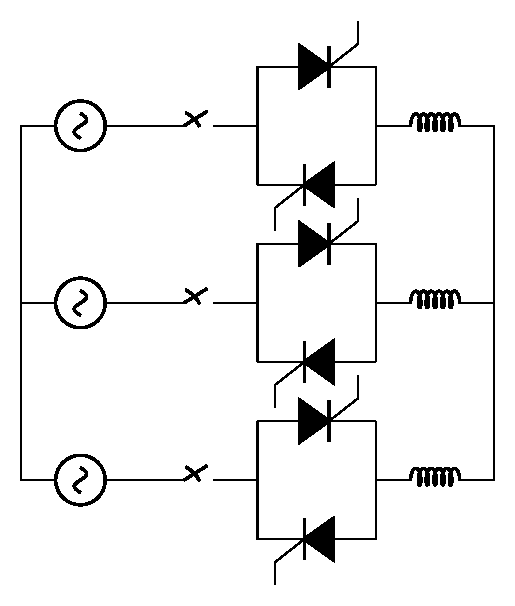
\includegraphics[scale=.45,angle=-90]{../sodomach/khoidongmem.pdf} 
		\end{center}
		
		\column{0.5\textwidth}
		\justifying
		Sử dụng \textcolor{red}{3 cặp SCR} để \textcolor{blue}{điều chỉnh điện áp} \textcolor{blue}{tăng áp} thông qua \textcolor{red}{góc kích} vào SCR rồi đưa giá trị điện áp điều chỉnh vào các cuộn dây stator của động cơ.
	\end{columns}
	\begin{block}{Đặc điểm}
		\justifying
		Thay đổi điện áp, giữ nguyên tần số.
		
		\begin{list}{--}{}
			\item Điện áp tăng từ giá trị đặt trước cho đến giá trị định mức.
			\item Điều chỉnh chính xác lực khởi động mong muốn.
			\item Điện áp hoạt động từ $200-500V$; tần số $f = 45-65Hz$.
		\end{list}
	\end{block}
\end{frame}

%--------------------------------------------------------------------------------
%--------------------------------------------------------------------------------
% Các phương pháp thay đổi tốc độ động cơ
\section[Thay đổi tốc độ động cơ KĐB ba pha]{Phương pháp thay đổi tốc độ động cơ KĐB ba pha}

%--------------------------------------------------------------------------------
% Tốc độ động cơ KĐB
\subsection{Thay đổi số cặp cực}
%--------------------------------------------------------------------------------
% Thay đổi số cặp cực
\begin{frame}{Phương pháp thay đổi tốc độ}
	\begin{block}{Phương pháp}
		\justifying
		\begin{list}{--}{}
			\item Mạch stator:
				\begin{list}{+}{}
					\item Thay đổi tần số nguồn cấp vào stator.
					\item Thay đổi số cặp cực dây quấn của stator.
					\item Thay đổi điện áp vào stator -- điều chỉnh hệ số trượt.
				\end{list}
			
			\item Mạch rotor: thay đổi điện trở để thay đổi hệ số trượt.
		\end{list}
	\end{block}
\end{frame}
\begin{frame}{Thay đổi số cặp cực}
	\begin{block}{Biện pháp}
		\justifying
		Thay đổi \textcolor{doden}{cấu tạo dây quấn}.
		\begin{list}{--}{}
			\item Thay đổi từng \textcolor{red}{cấp tốc độ không bằng phẳng}.
			\item \textcolor{blue}{Thay đổi cách nối dây} $\longrightarrow$ tạo số cặp cực khác nhau.
			\item Trên rãnh stator \textcolor{blue}{đặt 2 dây quấn độc lập có số đôi cực khác nhau}.
		\end{list}
   \end{block}
   \begin{block}{Phạm vi áp dụng}
   		\justifying
		Chỉ áp dụng cho động cơ \textcolor{doden}{rotor lồng sóc}.
		\begin{list}{--}{}
			\item \textcolor{red}{Số cặp cực} của \textcolor{blue}{rotor dây quấn} và \textcolor{blue}{stator} \textcolor{red}{bằng nhau} $\longrightarrow$ thay đổi dây quấn cả 2 nên \textcolor{red}{bất tiện}.
			\item \textcolor{blue}{Rotor lồng sóc} \textcolor{red}{thích ứng với số cặp cực} của \textcolor{blue}{stator}
		\end{list}
   \end{block}
\end{frame}

%--------------------------------------------------------------------------------
% Thay đổi điện áp stator
\subsection{Thay đổi điện áp stator}
\begin{frame}{Điều chỉnh điện áp nguồn cấp vào stator}
	\vspace{-2cm}
	\begin{center}
		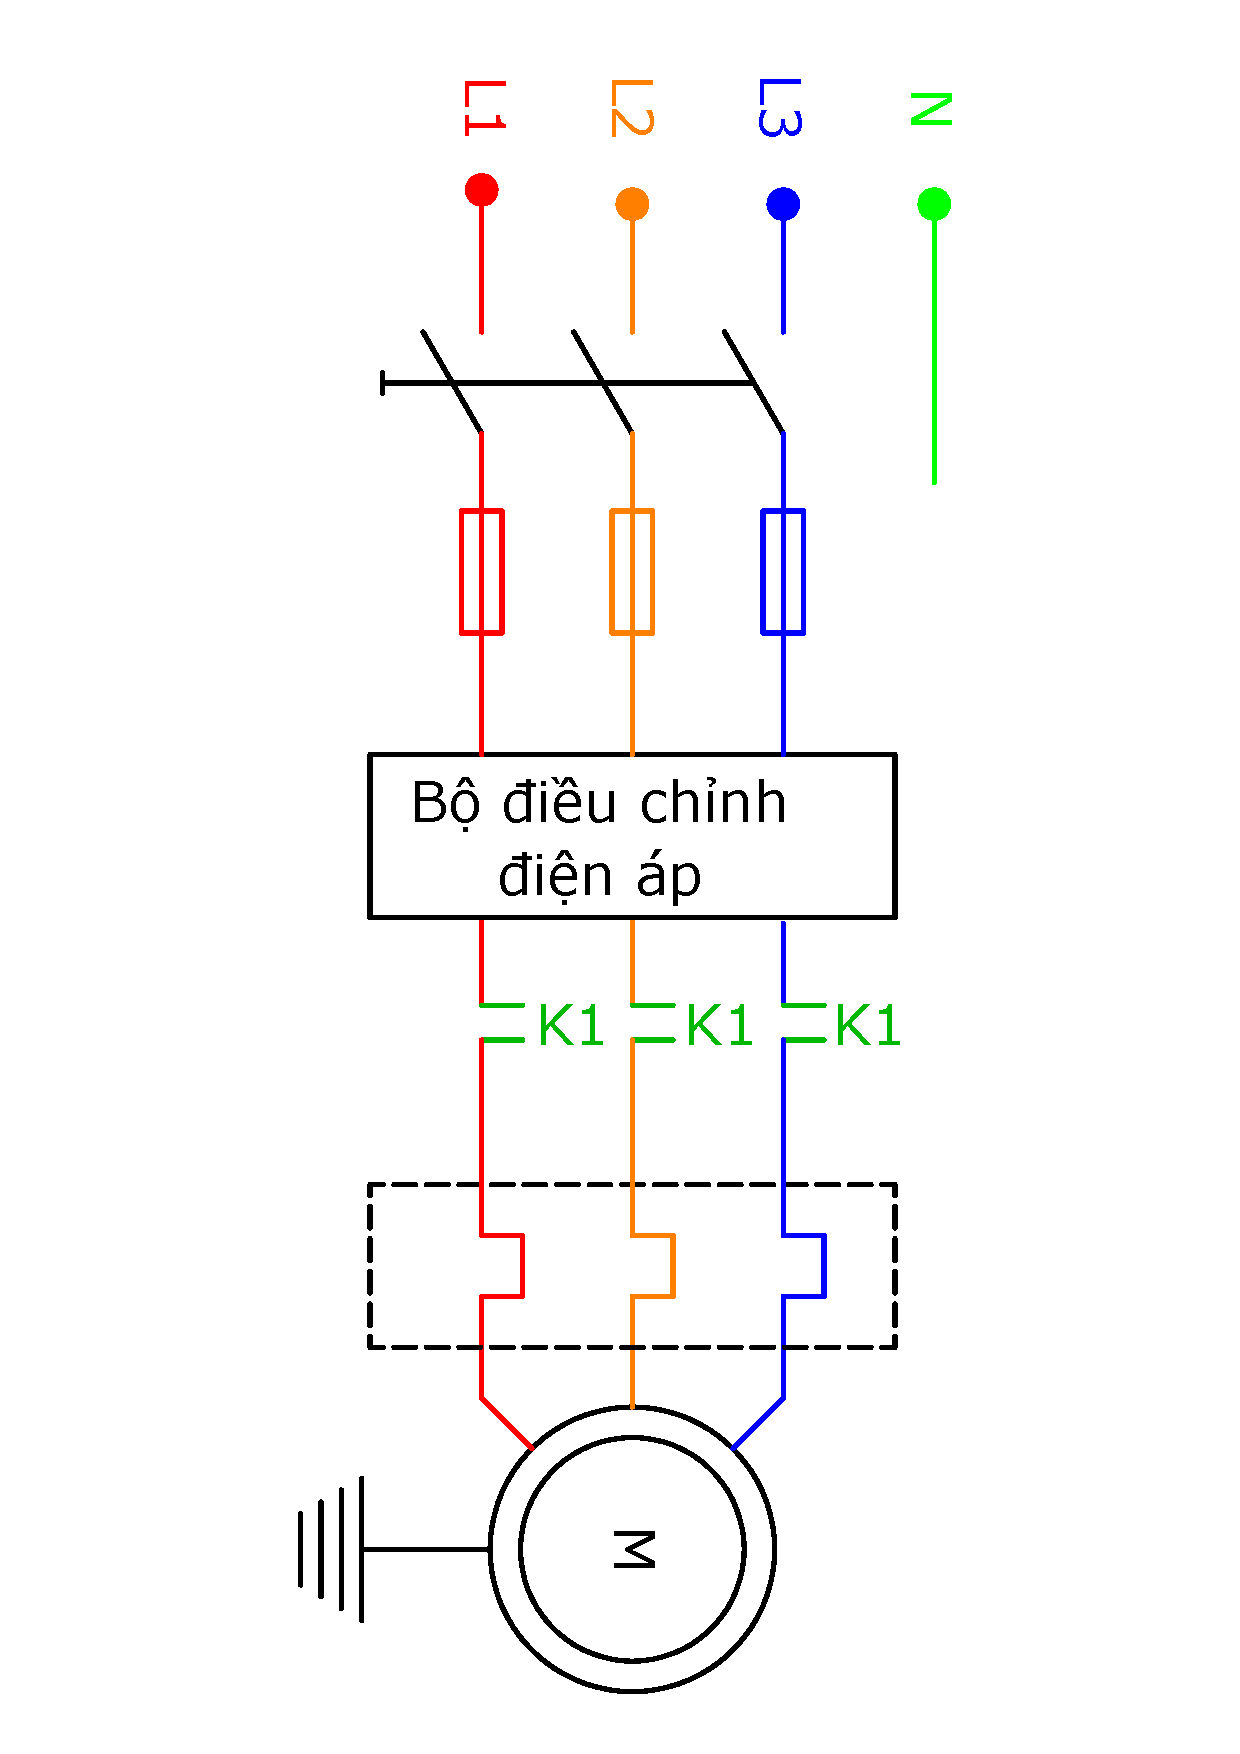
\includegraphics[scale=0.4, angle = 90]{../sodomach/dieu-chinh-dien-ap-stator.pdf}
	\vspace{-2cm}
	Bộ biến đổi điện áp: \textcolor{red}{bộ đổi điện}, \textcolor{red}{máy biến áp tự ngẫu}, \textcolor{red}{mạch SCR},\ldots
	\end{center}
\end{frame}

\subsection{Thay đổi điện trở mạch rotor}
\begin{frame}{Thay đổi điện trở mạch rotor}
	\vspace{-2.5cm}
	\begin{center}
		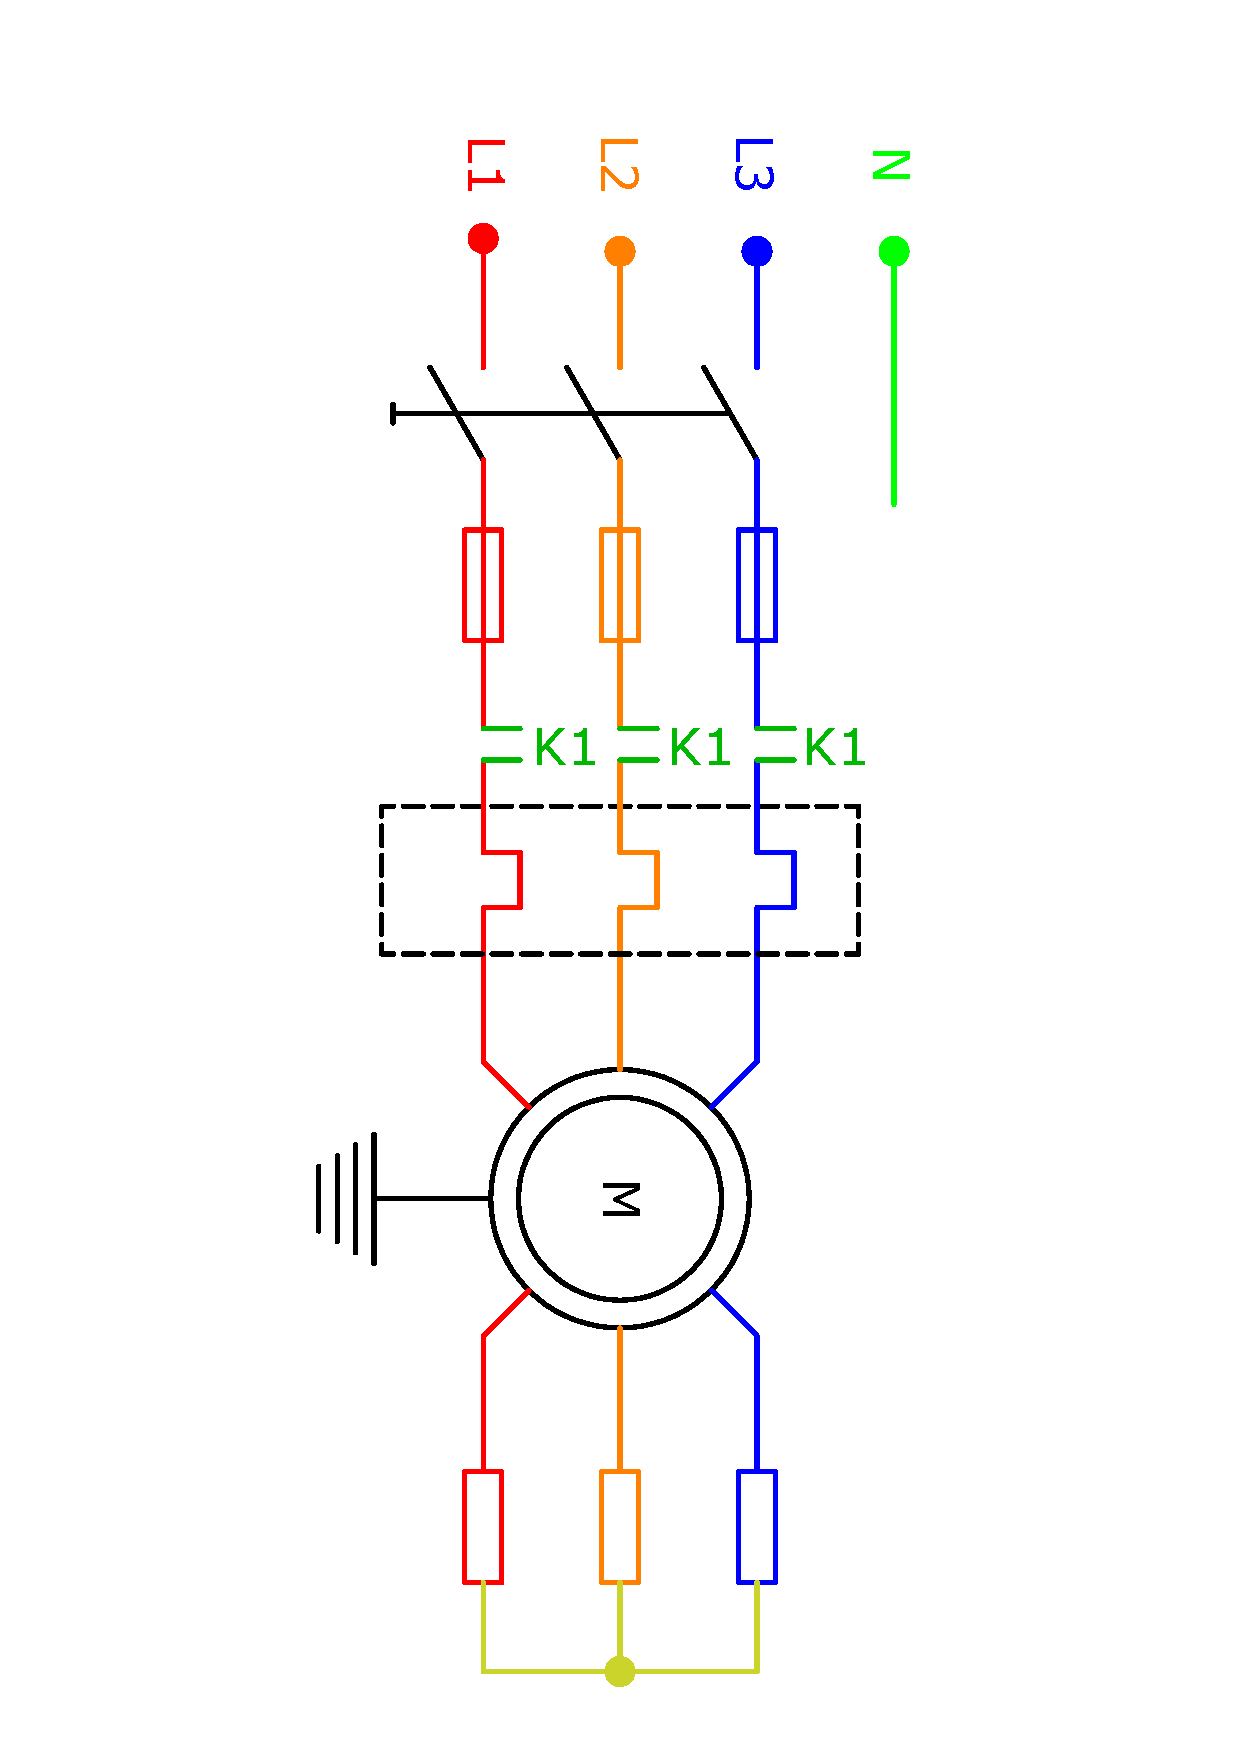
\includegraphics[scale=0.4, angle = 90]{../sodomach/dieu-chinh-dien-tro-rotor.pdf}
	\end{center}

	\vspace{-2.5cm}
	\begin{list}{--}{}
		\item Sử dụng 3 điện trở mắc vào 3 pha của động cơ.
		\item Giảm dòng điện vào động cơ $\longrightarrow$ tốc độ giảm theo.
	\end{list}
\end{frame}
\end{document}